\documentclass{beamer}
%
% Choose how your presentation looks.
%
% For more themes, color themes and font themes, see:
% http://deic.uab.es/~iblanes/beamer_gallery/index_by_theme.html
%
\mode<presentation>
{
   \usetheme{default}      % or try Darmstadt, Madrid, Warsaw, ...
   \usecolortheme{default} % or try albatross, beaver, crane, ...
   \usefonttheme{default}  % or try serif, structurebold, ...
   \setbeamertemplate{navigation symbols}{}
   \setbeamertemplate{caption}[numbered]
}

\usepackage[english]{babel}
\usepackage[utf8x]{inputenc}

% On writeLaTeX, these lines give you sharper preview images.
% You might want to comment them out before you export, though.
\usepackage{pgfpages}
\pgfpagesuselayout{resize to}[%
   physical paper width=8in, physical paper height=6in]

\title[Baseball Value]{Using Linear Regression to Find Value \\Players for Major League Teams} \author{Michael Scarinci\\Computational Methods for Analytics} \date{December 18th,2015}

\begin{document}

\begin{frame}
   \titlepage
\end{frame}

% Uncomment these lines for an automatically generated outline.
%\begin{frame}{Outline}
%  \tableofcontents
%\end{frame}

\section{Introduction}

\begin{frame}{Introduction}

\begin{block}{Preliminary Information}

\end{block}

\begin{itemize}
   \item  The average Major League Baseball player for 2015 will make \$4.25 Million. 
   \pause
   \item The Los Angeles Dodgers payroll for 2015 was over \$272 Million.
   \pause
   \item The world of Sabermetrics has redefined how teams find value in players.

\end{itemize}

\end{frame}

\begin{frame}{Important Stats to Know}

\begin{itemize}
	\item Runs Accounted Per Plate Appearance 
	\pause
	\item $\frac{Runs + RBI's - HR}{Plate Appearances}$
	\pause
	\item Batting Average and On Base Percentage (OBP)
	\pause
	\item wOBA, ISO, WAR, and wRC
	
\end{itemize}

\end{frame}

\section{Main Problem and Project Goals}

\subsection{Main Problem and Project Goals}

\begin{frame}{Main Problem and Project Goals}

\begin{block}{Main Problem}
\begin{itemize}


\item How can small market teams compete against large market teams?
\end{itemize}
\end{block}
\vspace{.75in}
\pause
\begin{block}{Project Goal}
\begin{itemize}
\item Find the best players to select based on percieved "underperformance" in the 2015 season.
\end{itemize}
\end{block}


% Commands to include a figure:
%\begin{figure}
%\includegraphics[width=\textwidth]{your-figure's-file-name}
%\caption{\label{fig:your-figure}Caption goes here.}
%\end{figure}

\end{frame}

\section{What Stats Should be Used}

\begin{frame}{Deciding the most predictable stat}

\begin{block}{wOBA had the highest $R^2$ value of .595, while Average had the lowest value with .1839}

\begin{figure}
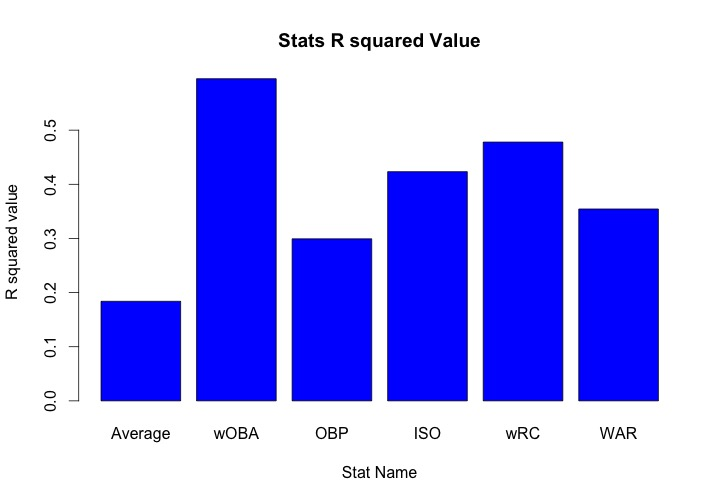
\includegraphics[width=3in]{Rsquared.jpeg}
\caption{\label{fig:your-figure}R squared value for each stat compared with RAPA.}
\end{figure}
\end{block}
\end{frame}


\begin{frame}{What can wOBA tell us?}

\begin{block}{The value of wOBA}

\begin{figure}
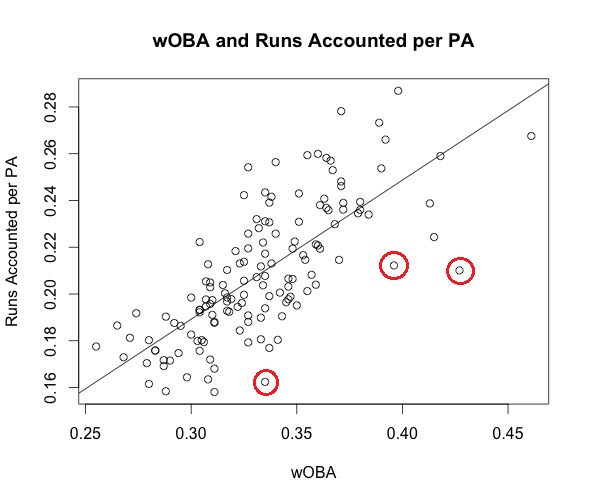
\includegraphics[width= 3 in]{wOBA.png}
\caption{Finding Value with wOBA.}
\end{figure}

\end{block}

\end{frame}

\begin{frame}{Value Players}

\begin{table}[]
\centering
\caption{Stats}
\label{my-label}
\begin{tabular}{|l|l|l|l|l|l|l|l|l|}
\hline
Player       & AVG  & wOBA & ISO  & OBP  & wRC & WAR & RA        \\ \hline
Joey Votto   & .314 & .427 & .228 & .459 & 172 & 7.4 & .210      \\ \hline
Nelson Cruz  & .302 & .396 & .264 & .369 & 158 & 4.8 & .212      \\ \hline
Joc Pederson & .210 & .335 & .206 & .346 & 115 & 2.8 & .162      \\ \hline
\end{tabular}
\end{table}

\end{frame}


\begin{frame}{Value Player's Team}
One reason for underperforming for 2015 was the entire team underperformed.

\begin{figure}
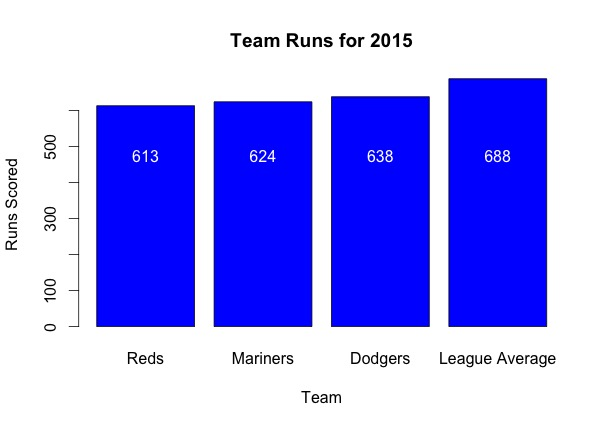
\includegraphics[width= 3 in]{TeamRuns.jpeg}
\caption{\label{fig:your-figure}Team's Runs versus League Average}
\end{figure}
\end{frame}


\begin{frame}{Finding the Best Model}
\begin{block}

What other stats should be used for determining their worth?\\
Leaps and regsubfit()\\
\begin{table}[]
\centering
\caption{Summary of regsubfit()}
\label{my-label}
\begin{tabular}{|c|c|c|c|c|c|c|}
\hline
Variables & wOBA & AVG & ISO & OBP & WAR & wRC \\ \hline
1         & *    &     &     &     &     &     \\ \hline
2         &      & *   & *   &     &     &     \\ \hline
3         & *    &     &     & *   &     & *   \\ \hline
4         & *    &     &     & *   & *   & *   \\ \hline
5         & *    & *   &     & *   & *   & *   \\ \hline
6         & *    & *   & *   & *   & *   & *   \\ \hline
\end{tabular}
\end{table}

\end{block}
\end{frame}


\begin{frame}{Selecting the best model}
Using all six variables will continuously increase our $R^2$ value.\\

\begin{figure}
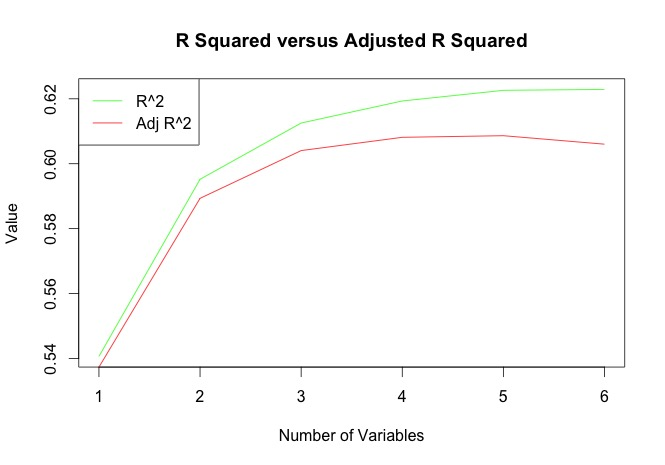
\includegraphics[width=3.3 in]{RvsadjR.jpeg}
\end{figure}

To avoid overfitting the data, I used adjusted $R^2$\\
Five variables gave the max adjusted $R^2$\\
\end{frame}


\begin{frame}{Equation}

\begin{center}
$\hat{y}$ $= -.082 + (1.551)wOBA + (.095)AVG -(.425)OBP$\\
 $+ (.002)WAR - (.001)wRC$
\end{center}

\end{frame}


\begin{frame}{Fit, Confidence and Prediction}

Using the model, the fit, confidence interval and prediction intervals were found.

\begin{table}[]
\begin{tiny}
\centering
\begin{tabular}{|c|c|c|c|c|c|c|}
\hline
\textbf{Player} & \textbf{Actual} & \textbf{Fit} & \textbf{CI Lower} & \textbf{CI Upper} & \textbf{Prediction Lower} & \textbf{Prediction Upper} \\ \hline
Joey Votto      & .210            & .249         & .236              & .261              & .212                      & .286                      \\ \hline
Nelson Cruz     & .212            & .248         & .239              & .258              & .212                      & .285                      \\ \hline
Joc Pederson    & .162            & .196         & .184              & .208              & .159                      & .233                      \\ \hline
\end{tabular}
\end{tiny}
\end{table}
\end{frame}

\begin{frame}{Using the Model}
\begin{block}{Player's Actual vs. Fit Runs Accounted for 2015}
\begin{figure}
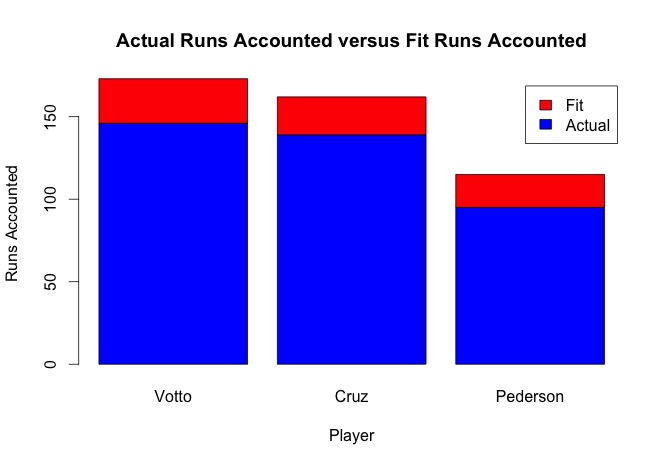
\includegraphics[width=\textwidth]{FitRuns.jpeg}
\caption{\label{fig:your-figure}Caption goes here.}
\end{figure}
\end{block}
\end{frame}

\begin{frame}{Taking Action}
\begin{block}{Nelson Cruz vs. Joey Votto}
Nelson Cruz made \$8 Million in 2015, when Votto made \$14 Million.
\end{block}
\pause
\begin{block}{What is Joc Pederson worth?}
At Joc Pederson's fit he would be equivalent to Melky Cabrera, who was paid \$8 Million.\\
\pause
Pederson's fit value was .196, compared to Cabrera's actual of .198 and fit .192.
\end{block}

\end{frame}

\begin{frame}{Summary}
\begin{block}{Further Exploration}
\begin{itemize}

\item Fielding
\pause
\item Age
\pause
\item Positional Value
\pause
\item Ball Park
\pause
\item Finding over valued players
\end{itemize}
\end{block}

\end{frame}

\begin{frame}
\begin{thebibliography}{1}

\bibitem{fangraphs} Baseball Statistics and Analysis | FanGraphs Baseball. Web. 17 Dec. 2015.

\bibitem{deadspin} Patchesky, Barry. "2015 Payrolls And Salaries For Every MLB Team." Deadspin. N.p., n.d. Web. 17 Dec. 2015.

\bibitem{stats}Dalgaard, Peter. Introductory Statistics with R. New York: Springer, 2002. 

\end{thebibliography}
\end{frame}

\begin{frame}
\begin{center}
\Huge Thank You
\end{center}
\end{frame}


\end{document}
